\section{Fabrication}\label{sec:fabrication}

The appealing theoretical predictions together with potential applications in logic, memory and sensor devices~\cite{Parkin08,Parkin15} determine the recent rapid development of fabrication methods for the needs of curvilinear ferromagnetism. To fabricate flat curvilinear systems it is important to rely on methods that provide preparation of magnetic samples with both predetermined material and geometrical properties.

\subsection{Geometrical construction}

To form a curved structure for the experimental investigation of the curvature-induced effects it is necessary to preserve an immutability of the structure's cross-section along a fabricated geometry. Therefore, it is required a lateral expansion of the wire along the unit vectors of the Frenet-Serret basis (Fig.~\ref{fig:Parabola_stripe_geometry}(a)), which allows to obtain a flat three-dimensional stripe with homogeneous geometrical properties: the curvature distribution is preserved as for a curvilinear
wire and cross-section along the stripe length is unchanged. The resulting shape is parametrized as follows
\begin{equation} \label{eq:Stripe_param}
\vec{r}(s,w,h) = \vec{\gamma}(s) + w \, \vec{e}_\textrm{N}(s) + h \, \vec{e}_\textrm{B}(s),
\end{equation}
where $w$ and $h$ being width $w \in [-W/2,W/2]$ and thickness $h \in [-H/2,H/2]$ of the stripe, respectively, see Fig.~\ref{fig:Parabola_stripe_geometry}(c) and (d). When the stripe is constructed in this way, the shape parameters remain unchanged within the Frenet-Serret basis up to the critical curvature $\kappa^\textrm{c}_0 = 2/W$. For $\kappa_0>\kappa^\textrm{c}_0$, there appears widening in the central part of the stripe due to the overlap of parabolic branches, Fig.~\ref{fig:Parabola_stripe_geometry}(b).

\begin{figure*}
	\begin{center}
		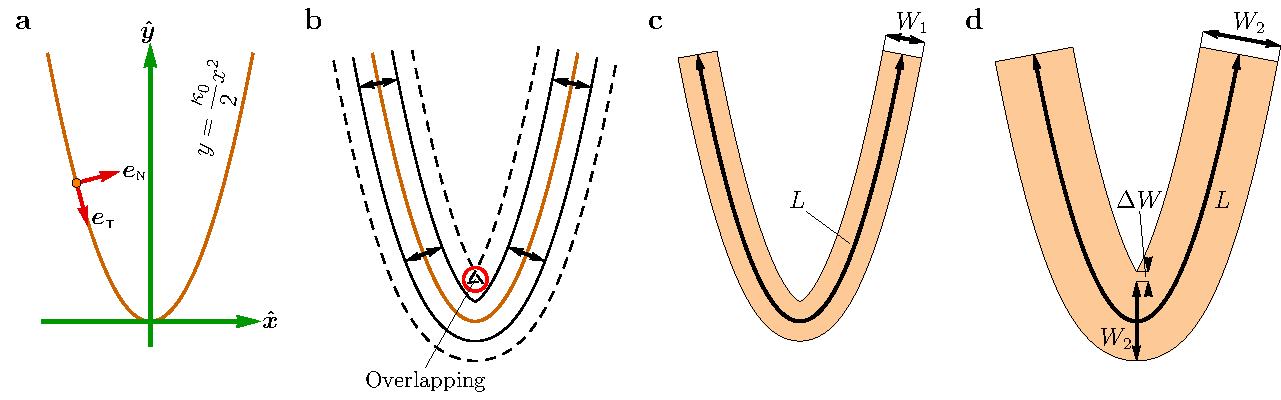
\includegraphics[width=0.9\linewidth]{fig_stripe_construction.pdf}
	\end{center}
	\caption{\textit{Geometrical construction of a parabolic stripe.}~(a), One-dimensional parabolic wire in a Cartesian frame of reference.~(b), Schematic picture of a parabolic stripe geometry construction from one-dimensional wire expansion along the normal direction $\vec{e}_\textrm{N}$.~(c) and (d), Show the resulting stripe geometries with two different widths $W_1$ and $W_2=2 W_1$, respectively. Local widening in the apex area of the parabolic stripe is indicated by $\Delta W$.}
	\label{fig:Parabola_stripe_geometry}
\end{figure*}	

\subsection{Lithographic methods}

Standard lithographic techniques combined with thin film deposition represent the first group of methods, that allow to fabricate two-dimensional curved magnetic objects. One of the most developed techniques among this group is Electron Beam Lithography (EBL) method, which allows to ensure shape retention of the patterned geometry and achieve high spatial resolution down to dozens of nanometers. A typical EBL system contains a precise emission source of electrons and necessary optics for the control and focusing of electron beam. The predetermined shape of the object is drawn in a electron-sensitive resist, whose solubility is changing under the electron beam exposure. This enables it selective removal of either the exposed (positive resist), or non-exposed (negative resist) regions of the resist by immersing it in a chemical developer. The remaining parts of the resist are using either for filling the remaining spaces between them with required material composition, or as a protection of the initially deposited layers from ion-beam etching. The resulting nanostructure could be revealed by removing the remaining resist in a specific solvent. This approach provided the opportunity to study magnetic processes in curved nanostripes~\cite{Lewis09,Nahrwold09,Glathe12} and nanorings~\cite{Klaui03a,Klaui05a,Klaui08,Richter16,Mawass17}  to address DW dynamics and automotion~\cite{Mawass17} for prospective memory~\cite{Hayashi07,Parkin08,Parkin15} and logic~\cite{Allwood02,Allwood04,Allwood05,Hrkac11} devices, as well as the concept of magnon-based processing of binary data~\cite{Schneider08,Lee08e,Vogt12,Vogt14,Chumak15}.


\subsection{Ion-induced methods}

\textit{Direct 2D writing} through the irradiation of B2-A2 phase alloys (e.g. FeAl alloy~\cite{Bali14}) allows to reach the element spatial resolution at the same or better level than lithography-based approaches. This method is based on thin films that are paramagnetic after preparation (B2 phase), but obtain ferromagnetic order after the irradiation due to the induced chemical disorder (A2 phase). As shown recently~\cite{Nord19}, using He$^{+}$ or Ne$^{+}$ irradiation in He-ion microscope it is possible to write into FeAl flat curvilinear magnetic nanostructures with a 2~nm precision.

%/-----------------------------------------------------------------------------------------
%
%Recent progress in material science enabled the appearance of various microscale additive manufacturing technologies, that provide the ability to build 3D curvilinear geometries that are not limited by the conventional lithographic or specific layer growth techniques~\cite{Hirt17}. One of the most prominent techniques of additive manufacturing of magnetic materials is focused electron-beam induced deposition (FEBID)~\cite{Teresa16,Huth18,Fernandez-Pacheco20} which in the recent years has reached a high level of maturity for the fabrication of complex-shaped 3D nano-architecures \cite{Keller18,Winkler19,Skoric20,Sanz-Hernandez20,Hunt20}. FEBID is based on the beam-induced dissociation of precursor organic molecules with the resulting non-volatile leftovers, that form a predetermined curvilinear geometry. The resulting self-standing magnetic geometries could be of any complex shape~\cite{Fernandez17}: self-standing magnetic nanostripes~\cite{Sanz-Hernandez17}, see Fig.~\ref{Fig:Experimental_figs_1}(g), nanoscale double-helix structures~\cite{Sanz-Hernandez20}, nano-cubes with nano-trees~\cite{Keller18,Mamoori18,Huth18} and nano-amphora~\cite{Huth20}. The two-photon lithography is another additive technology that allows to create sub-$\mu$m size self-standing curvilinear objects of various shapes that could be covered with magnetic materials~\cite{Williams18,Sahoo18,May19,Hunt20}, see Fig.~\ref{Fig:Experimental_figs_1}(h). This enables ``writing'' of almost arbitrary geometries and magnetic materials, which leads to the rapid prototyping of complex magnetic curvilinear geometries. 
